\documentclass[aspectratio=169]{beamer}

\usepackage{ccicons}
\usepackage{fontspec}
\usepackage{listings}
\usepackage{tikz}
\usepackage{svg}

\definecolor{uclablue}{RGB}{39,116,174}
\definecolor{uclagold}{RGB}{255,179,0}

\definecolor{ubcorange}{RGB}{158, 66, 37}

\definecolor{cugold}{RGB}{207, 184, 124}
\definecolor{cudarkgray}{RGB}{86, 90, 92}

\definecolor{solarizedred}{RGB}{220, 50, 47}
\definecolor{solarizedblue}{RGB}{38, 139, 210}
\definecolor{solarizedgreen}{RGB}{133, 153, 0}
\definecolor{solarizedpurple}{RGB}{108, 113, 196}
\definecolor{solarizedmagenta}{RGB}{211, 54, 130}

\definecolor{pantone655}{RGB}{0, 42, 92}
\definecolor{pantone7453}{RGB}{123, 164, 217}
\definecolor{pantone633}{RGB}{0, 139, 176}
\definecolor{pantone7492}{RGB}{218, 229, 205}

\colorlet{primarycolor}{pantone655}
\colorlet{secondarycolor}{pantone7453}


\usetikzlibrary{
  arrows,
  arrows.meta,
  automata,
  backgrounds,
  calc,
  chains,
  decorations.pathreplacing,
  fit,
  intersections,
  matrix,
  overlay-beamer-styles,
  positioning,
  shapes,
  shapes.multipart,
  tikzmark,
}
\usetikzmarklibrary{listings}

\hypersetup{
  colorlinks=true,
  urlcolor=cudarkgray,
}

\setbeamercolor{frametitle}{fg=primarycolor}
\setbeamercolor{structure}{fg=primarycolor}
\setbeamercolor{enumerate item}{fg=black}
\setbeamercolor{itemize item}{fg=black}
\setbeamercolor{itemize subitem}{fg=black}

\setbeamersize{text margin left=26.6mm}
\addtolength{\headsep}{2mm}

\setbeamertemplate{navigation symbols}{}
\setbeamertemplate{headline}{}
\setbeamertemplate{footline}{}
\setbeamertemplate{itemize item}{\color{black}}
\setbeamertemplate{itemize items}[circle]

\setbeamertemplate{footline}{
  \begin{tikzpicture}[remember picture,
                      overlay,
                      shift={(current page.south west)}]
    \node [black!50, inner sep=2mm, anchor=south east]
          at (current page.south east) {\footnotesize \insertframenumber};
  \end{tikzpicture}
}

\setsansfont{Inter}[Scale=MatchLowercase]
\setmonofont{Hack}[Scale=MatchLowercase]

\makeatletter
\newcommand\version[1]{\renewcommand\@version{#1}}
\newcommand\@version{}
\def\insertversion{\@version}

\newcommand\lecturenumber[1]{\renewcommand\@lecturenumber{#1}}
\newcommand\@lecturenumber{}
\def\insertlecturenumber{\@lecturenumber}
\makeatother

\setbeamertemplate{title page}
{
  \begin{tikzpicture}[remember picture,
                      overlay,
                      shift={(current page.south west)},
                      background rectangle/.style={fill=pantone655},
                      show background rectangle]
    \node [anchor=west, align=left, inner sep=0, text=white]
          (lecturenumber) at (\paperwidth / 6, \paperheight * 3 / 4)
          {\Large Lecture \insertlecturenumber};
    \node [inner sep=0, align=left, text=white, node distance=0,
          above left=of lecturenumber, anchor=south west, yshift=2mm]
          {\Large ECE 344: Operating Systems};
    \node (title) [inner sep=0, anchor=west, align=left, text=white,
                   text width=30em]
          at (\paperwidth / 6, \paperheight / 2)
          {{\bfseries \Huge \inserttitle{}}};
    \node [inner sep=0, align=right, text=white, node distance=0,
          below right=of title, anchor=north east, yshift=-1mm]
          {{\footnotesize \ttfamily \insertversion}};
    \node [inner sep=0, text=white, align=left, anchor=west]
          (author) at (\paperwidth / 6, \paperheight / 4)
          {\insertauthor};
    \node [text=white, inner sep=0, align=left, node distance=0,
           below left=of author, anchor=north west, yshift=-2mm]
          {\insertdate};
    \node [align=right, anchor=south east, inner sep=2mm, text=white]
          (license) at (\paperwidth, 0)
          {\footnotesize This  work is licensed under a
           \href{http://creativecommons.org/licenses/by-sa/4.0/}
                {\color{pantone7453} Creative Commons Attribution-ShareAlike 4.0
                 International License}};
    \node [text=white, inner sep=0, align=right, node distance=0,
           above right=of license, anchor=south east, xshift=-2mm]
          {\Large \ccbysa};
  \end{tikzpicture}
}

\tikzset{
  >=Straight Barb[],
  shorten >=1pt,
  initial text=,
}

\lstset{
  basicstyle=\footnotesize\ttfamily,
  language=C,
  escapechar=@,
  commentstyle=\color{black!50},
}


\lecturenumber{8}
\title{Threads Implementation}
\version{1.1.1}
\author{Jon Eyolfson}
\date{September 26, 2022}

\begin{document}
  \begin{frame}[plain, noframenumbering]
    \titlepage
  \end{frame}

  \begin{frame}
    \frametitle{Multithreading Models}

    Where do we implement threads?

    \hspace{2em} We can either do user or kernel threads

    \vspace{2em}

    User threads are completely in user-space

    \hspace{2em} Kernel doesn't treat your threaded process any differently

    \vspace{2em}

    Kernel threads are implemented in kernel-space

    \hspace{2em} Kernel manages everything for you, and can treat threads specially
  \end{frame}

  \begin{frame}
    \frametitle{Thread Support Requires a Thread Table}

    Similar to the process table we saw previously

    \hspace{2em} It could be in user-space or kernel-space depending

    \vspace{2em}

    For user threads, there also needs to be a run-time system to determine
    scheduling

    \vspace{2em}

    In both models each process can contain multiple threads
  \end{frame}

  \begin{frame}
    \frametitle{We Could Avoid System Calls, or Let a Thread Block Everything}

    For pure user-level threads (again, no kernel support):

    \begin{itemize}
      \item Very fast to create and destroy, no system call, no context switches
      \item One thread blocks, it blocks the entire process (kernel can't distinguish)
    \end{itemize}

    \vspace{2em}

    For kernel-level threads:

    \begin{itemize}
      \item Slower, creation involves system calls
      \item If one thread blocks, the kernel can schedule another one
    \end{itemize}
  \end{frame}

  \begin{frame}
    \frametitle{All Threading Libraries You Use Run in User-mode}

    The thread library maps user threads to kernel threads

    \vspace{2em}

    Many-to-one: threads completely implemented in user-space

    \hspace{2em} the kernel only sees one process

    \vspace{2em}

    One-to-one: one user thread maps directly to one kernel thread

    \hspace{2em} the kernel handles everything

    \vspace{2em}

    Many-to-many: many user-level threads map to many kernel level threads
  \end{frame}

  \begin{frame}
    \frametitle{Many-to-one is Pure User-space Implementation}

    It's fast (as outlined before) and portable

    \hspace{2em} It doesn't depend on the system, it's just a library

    \vspace{2em}

    Drawbacks are that one thread blocking causes all threads to block

    \hspace{2em} Also we cannot execute threads in parallel

    \hspace{4em} The kernel will only schedule a process to run
  \end{frame}

  \begin{frame}
    \frametitle{One-to-one Just Uses the Kernel Thread Implementation}

    There's just a thin wrapper around the system calls to make it easier to use

    \vspace{2em}

    Exploits the full parallelism of your machine

    \hspace{2em} The kernel can schedule multiple threads simultaneously

    \vspace{2em}

    We do however need to use a slower system call interface,
    
    \hspace{2em} and we lose some control

    \vspace{4em}

    Typically this is the actual implementation used, we'll assume this for
    Linux
  \end{frame}

  \begin{frame}
    \frametitle{Many-to-many is a Hybrid Approach}

    The idea is that there are more user-level threads than kernel-level threads

    \hspace{2em} Cap the number of kernel-level threads to the number we could
    run in parallel

    \vspace{2em}

    We can get the most out of multiple CPUs and reduce the number of system
    calls

    \vspace{2em}

    However, this leads to a complicated thread library

    \hspace{2em} Depending on your mapping luck, you may block other threads
  \end{frame}

  \begin{frame}
    \frametitle{Threads Complicate the Kernel}

    How should \texttt{fork} work with a process with multiple threads?

    \hspace{2em} Copy all threads to the new process, in whatever state they're
    in?

    \hspace{4em} How would this get out of hand?

    \vspace{2em}

    Linux only copies the thread that called \texttt{fork} into a new process

    \hspace{2em} If it hits \texttt{pthread\_exit} it'll always exit with status
    0

    \hspace{4em} (at least as far as I can tell)

    \vspace{2em}

    There's \texttt{pthread\_atfork} (not covered in this course) to control
    what happens
  \end{frame}

  \begin{frame}
    \frametitle{Signals are Sent to a Process}

    Which thread should receive a signal? all of them?

    \vspace{2em}

    Linux will just pick one random thread to handle the signal

    \hspace{2em} Makes concurrency hard, any thread could be interrupted
  \end{frame}

  \begin{frame}
    \frametitle{Instead of Many-to-many, You Can Use a Thread Pool}

    The goal of many-to-many thread mapping is to avoid creation costs

    \vspace{2em}

    A thread pool creates a certain number of threads and a queue of tasks

    \hspace{2em} (maybe as many threads as CPUs in the system)

    \vspace{2em}

    As requests come in, wake them up and give them work to do

    \vspace{2em}

    Reuse them, when there's no work, put them to sleep
  \end{frame}

  \begin{frame}
    \frametitle{You'll Implement Many-to-one}

    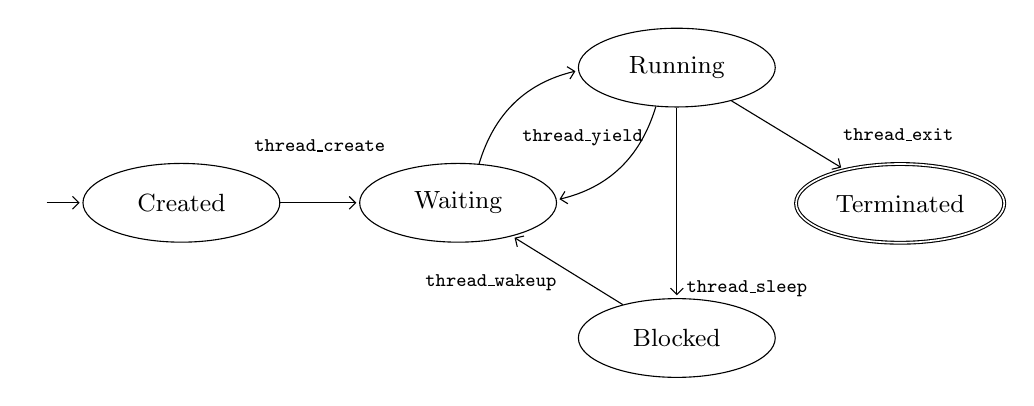
\begin{tikzpicture}[
      every state/.style={ellipse, minimum width=2.5cm, minimum height=1cm, font=\small},
    ]
      \node [state, initial] (created) {Created};
      \node [state, right=of created] (waiting) {Waiting};
      \node [state, above right=of waiting] (running) {Running};
      \node [state, below right=of waiting] (blocked) {Blocked};
      \node [state, accepting, below right=of running] (terminated) {Terminated};
      \path [->] (created) edge (waiting) node [above, xshift=5em, yshift=1.5em] {\scriptsize \ttfamily thread\_create}
                 (waiting) edge [bend left] (running) node [below, xshift=4.5em, yshift=3em] {\scriptsize \ttfamily thread\_yield}
                 (running) edge [bend left] (waiting)
                 (running) edge (blocked) node [right, yshift=-8em] {\scriptsize \ttfamily thread\_sleep}
                 (blocked) edge (waiting) node [left, xshift=-4em, yshift=2em] {\scriptsize \ttfamily thread\_wakeup}
                 (running) edge (terminated) node [above, xshift=8em, yshift=-3em] {\scriptsize \ttfamily thread\_exit};
    \end{tikzpicture}
  \end{frame}

  \begin{frame}
    \frametitle{Your Scheduler Can Just Be Round Robin}

    Create a queue (list), run the thread at the front, when it yeilds at it to the back

    \vspace{2em}

    You'll have to do the context switch (remember, you'll have to save the registers)

    \vspace{2em}

    These are cooperative threads, so they have to be nice (next is preemptive threads)
  \end{frame}

  \begin{frame}
    \frametitle{Our Next Complication}

    Let's create a program that spawns 8 threads

    \hspace{2em} Each thread increments the same variable 10,000 times

    \vspace{2em}

    What should the final value of the variable be?

    \hspace{2em} The initial value of the variable is 0

    \vspace{2em}

    Run \texttt{lecture-08/pthread-datarace}

    \hspace{2em} Can you fix it?
  \end{frame}

  \begin{frame}
    \frametitle{Both Processes and (Kernel) Threads Enable Parallelization}

    \begin{itemize}
      \item Each process can have multiple (kernel) threads
      \item Most implementations use one-to-one user-to-kernel thread mapping
      \item The operating system has to manage what happens during a fork, or signals
      \item We now have synchronization issues
    \end{itemize}
  \end{frame}
\end{document}
